\section{Experimental Setup}

\subsection*{Circuit components}
    \begin{enumerate}
        \item Transistor (CL100 or equivalent)
        \item Power supply
        \item 6 resistors of various specifications
        \item 3 Capacitors 
        \item Function Generator
        \item Oscilloscope
        \item Multimeters
        \item Connecting wires
        \item Breadboard
    \end{enumerate}

    \subsection*{Circuit Diagram}
    \begin{figure}[H]
        \centering
        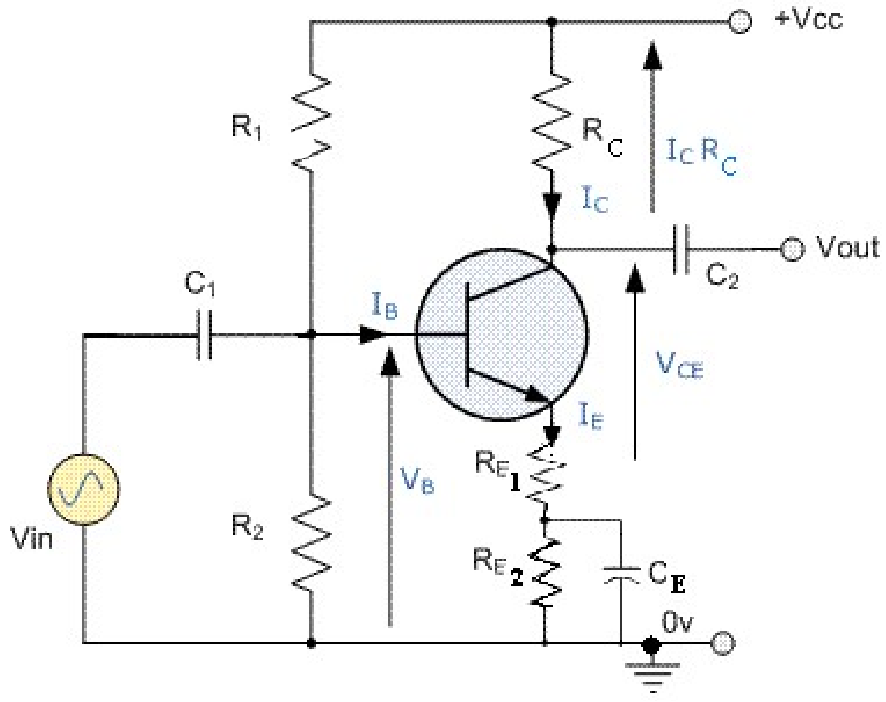
\includegraphics[width=0.8\columnwidth]{images/f1.png}
        \caption{Circuit diagram for the setup.}
        \label{fig:1}
    \end{figure}

\section{Data Analysis}

\begin{itemize}
    \item $V_{CC} = 12$ V
    \item $V_i$ (pp) = 200 mV
    \item $\beta = 168$
    \item $R_1=26.81\,k\Omega$
    \item $R_2=(4.65+0.222)=4.872\,k\Omega$
    \item $R_C=3.849\,k\Omega$
    \item $R_{E1}=0.4678\,k\Omega$, $R_{E2}=0.5624\,k\Omega$, hence $R_E=1.03\,k\Omega$
    \item $C_1=1.017\,\mu$F, $C_2=0.985\,\mu$F
    \item $C_E=95.4\,\mu$F\\
\end{itemize}

We measured the following values from the D.C. analysis of the circuit.

\begin{table}[H]
    \centering
    \begin{tabular}{|c|c|c|}
    \hline
    Parameter & Computed Value & Observed Value \\ \hline
    $V_B$ (V) & 1.845  &  1.808 \\
    $V_E$ (V) & 1.145  &  1.216 \\
    $I_C\approx I_E$ (mA) & 1.11 & 1.19 \\
    $V_{CE}$ (V) & 6.57 & 6.19 \\
    \hline
    \end{tabular}
    \caption{D.C. analysis of the circuit}
    \label{tab:1}
\end{table}

From Table \ref{tab:1}, we can find the Q-point of the circuit as (6.19 V, 1.19 mA).

Hence, $r_e=26$mV$/I_E=21.85\,\Omega$.
From Eq. (7),
\begin{align*}
    Z_i &= R_1 \parallel R2 \parallel \beta r_e \\
    &= \left( \frac{1}{26810}+\frac{1}{4872}+\frac{1}{168\cross 21.85} \right)^{-1} \\
    &= 1.941\,\text{k}\Omega
\end{align*}

Similarly,

\begin{align*}
    Z_o &= R_C \parallel r_o \\
    &= \left( \frac{1}{R_C}+\frac{1}{r_o}\right)^{-1} \\
    &\approx R_C=3.849\,\text{k}\Omega
\end{align*}

Since $r_o$ is is the range of $\sim$ 100 k$\Omega$, we can ignore it.

Also, we can find the theoretical value of $A_V$ in mid-frequency range from Eq. (9),

\begin{align*}
    A_V &= \frac{3849}{467.8+21.85} = 7.861\\
    \text{or, Gain }&= 17.91\,\text{dB}
\end{align*}

Here is the plot of the frequency response curve of the circuit.
\begin{figure}[H]
    \centering
    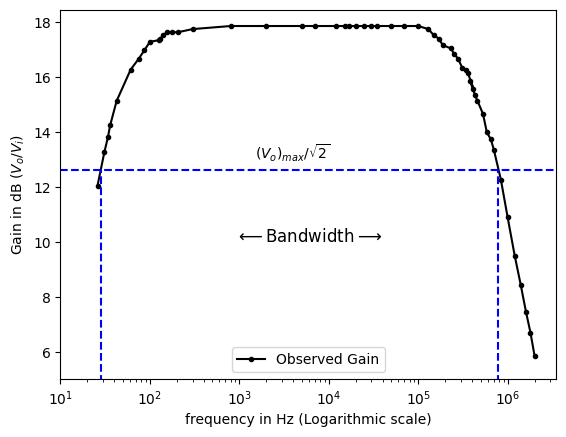
\includegraphics[width=1\columnwidth]{images/g1.png}
    \caption{Frequency response curve: $A_V$ vs. frequency plot}
    \label{graph}
\end{figure}

From Fig. \ref{graph}, we can estimate the following values,

\begin{itemize}
    \item Mid frequency Gain: 17.84 dB (or $V_o/V_i=7.8$)
    \item Cut-off frequencies: 28.58 Hz and 784.16 kHz and 
    \item Mid-frequency range: 800 Hz to 100 kHz and 
    \item Bandwidth: 784.13 kHz
\end{itemize}